\documentclass[conference]{IEEEtran}
\usepackage[utf8]{inputenc}
\usepackage{float}
\usepackage{enumitem}
\usepackage{balance}
\usepackage[hang,flushmargin]{footmisc}
\usepackage{lipsum}
\usepackage{graphicx}
\usepackage{hyperref}
\usepackage{amsmath}
\usepackage{array}
\usepackage{booktabs}
\usepackage{multirow}

\title{Time Series Forecasting Using Deep Learning: A Case Study on Walmart Sales Data}

\author{
\IEEEauthorblockN{
Tamanna Sharma,
Jenny Prasad,
Ashish Pal,
Piyush Takrani,
Khushdeep Singh,
Arham Khan}
}

\begin{document}

\maketitle  % ✅ Only one maketitle

% ✅ Centered Supervisor block after maketitle
\vspace{1.5em}
\begin{center}
\textbf{Supervisor: Dr. Sangeeta Yadav}\\
Faculty Of Technology, University Of Delhi\\
\end{center}
\vspace{1em}

% Title block
\title{Time Series Forecasting Using Deep Learning: A Case Study on Walmart Sales Data}



% Front Page


\begin{abstract}
This project investigates the application of deep learning models for time series forecasting, focusing specifically on predicting weekly retail sales using Walmart's dataset. The dataset includes historical sales records, promotional features, and store metadata across various locations and departments. We employ two powerful recurrent neural network architectures—Long Short-Term Memory (LSTM) and Gated Recurrent Unit (GRU)—to model temporal dependencies and forecast future sales. Key preprocessing steps included merging and aligning multiple data sources, normalizing the target variable, and generating sliding input sequences based on varying historical time windows. Experimental evaluations were conducted across five dimensions: varying sequence lengths, incorporating different feature combinations, attempting alternative prediction targets, experimenting with LSTM architecture complexity (layers and neurons), and comparing the predictive performance of LSTM and GRU models. Our results demonstrate that deep learning models, particularly GRU, provide accurate and reliable forecasts, validating their effectiveness over traditional time series methods in complex retail environments. Libraries such as TensorFlow, Keras, and scikit-learn were utilized for model implementation and evaluation. Dataset sizes include a training set of shape (421570, 5), a features set of shape (8190, 12), and a store metadata set of shape (45, 3).
\end{abstract}

\section{Introduction}
Time series forecasting is a widely-used technique in machine learning and data science, involving the prediction of future values based on previously observed data points ordered over time. It finds critical applications in sectors such as finance, healthcare, weather prediction, energy consumption, and retail analytics. Traditional statistical methods like ARIMA and SARIMA have long been used to forecast time series data; however, they often fall short in capturing complex non-linear dependencies and interactions over long temporal windows.

Retail sales forecasting, in particular, presents unique challenges due to the complex interplay of factors affecting consumer behavior. These include seasonality patterns, promotional events, economic indicators, competition, and even weather conditions. Accurate forecasting is crucial for retailers to optimize inventory management, staffing decisions, supply chain operations, and marketing strategies. In large retail operations like Walmart, even small improvements in forecasting accuracy can translate to significant cost savings and competitive advantages.

The advent of deep learning approaches has revolutionized time series forecasting by offering powerful alternatives to traditional statistical methods. Recurrent Neural Networks (RNNs), particularly their variants such as Long Short-Term Memory (LSTM) and Gated Recurrent Unit (GRU) networks, have demonstrated remarkable capabilities in capturing complex temporal patterns and long-range dependencies in sequential data. These architectures incorporate specialized mechanisms to address the vanishing gradient problem that plagued earlier RNN implementations, enabling them to learn from extended historical sequences.

This study aims to apply and evaluate deep learning-based forecasting techniques on a real-world dataset from Walmart. The dataset includes historical weekly sales data, store features, and promotional information across various departments and locations. The multi-dimensional nature of this dataset—spanning different stores, departments, and time periods—provides an ideal testing ground for assessing the capabilities of advanced neural network architectures in real-world retail forecasting scenarios.

Our research is motivated by several key questions:
\begin{itemize}
  \item How does the historical sequence length affect forecasting accuracy, and what is the optimal window size for retail sales prediction?
  \item Which combinations of features (economic indicators, store characteristics, promotional information) yield the most accurate sales forecasts?
  \item How do different neural network architectures compare in terms of forecasting performance and computational efficiency?
  \item Can deep learning models maintain consistent performance across different temporal segments and forecasting horizons?
  \item What architectural configurations and hyperparameter settings maximize prediction accuracy while maintaining generalization capability?
\end{itemize}

To address these questions, our methodology involves five core experiments: (1) evaluating the impact of sequence length on model accuracy, (2) engineering different feature combinations to improve performance, (3) exploring alternative forecasting targets beyond the immediate next week, (4) testing different LSTM model complexities by altering the number of layers and neurons, and (5) comparing the performance of LSTM and GRU networks. Additionally, we conduct a segment-wise error analysis to investigate performance variations across different temporal periods. The performance of each model is measured using standard error metrics such as Mean Absolute Error (MAE) and Root Mean Squared Error (RMSE).

The insights gained from this research have significant practical implications for retailers seeking to leverage deep learning for sales forecasting. By systematically evaluating various aspects of model design and implementation, we aim to provide actionable guidelines for developing effective forecasting systems that can accommodate the complex, multi-faceted nature of retail sales data. Furthermore, our findings contribute to the broader understanding of deep learning applications in time series analysis, particularly in contexts involving multiple interacting factors and hierarchical data structures.

\section{Literature Review}
Accurate sales forecasting is crucial for efficient inventory management, resource allocation, and strategic decision-making in large-scale retail operations like Walmart. This section provides a comprehensive review of the evolution of forecasting methodologies, from traditional statistical approaches to contemporary deep learning techniques, with a particular focus on their application in retail contexts.

\subsection{Traditional Time Series Forecasting Methods}
Time series forecasting has historically relied on statistical methods that decompose historical data into trend, seasonal, and residual components. These approaches include moving averages, exponential smoothing, and autoregressive integrated moving average (ARIMA) models. Hyndman \& Athanasopoulos (2018) provide a comprehensive overview of these techniques, highlighting their mathematical foundations and practical applications.

The ARIMA family of models, including seasonal variants (SARIMA), has been widely used in retail forecasting due to their ability to capture linear relationships and certain forms of seasonality. However, Zhang (2003) demonstrated that these traditional methods often struggle to capture the complex non-linear patterns, long-range dependencies, and the impact of exogenous factors inherent in retail datasets. This limitation is particularly pronounced in environments characterized by volatile demand patterns, frequent promotional activities, and external economic influences—all common features in modern retail settings.

Extensions to traditional methods have attempted to address these limitations. For instance, ARIMAX and regression models with ARIMA errors incorporate external variables, while state space models provide more flexible frameworks for handling complex seasonal patterns. Despite these advancements, Box et al. (2015) noted that such methods still rely on assumptions of linearity and stationarity that may not hold in real-world retail scenarios.

\subsection{Machine Learning Approaches to Time Series Forecasting}
The limitations of traditional statistical methods led to the exploration of machine learning techniques for time series forecasting. Support Vector Machines (SVMs), Random Forests, and Gradient Boosting have demonstrated promising results in various forecasting applications. These methods offer greater flexibility in capturing non-linear relationships without requiring explicit specification of the underlying data generation process.

Crone et al. (2011) conducted a comparative study of machine learning methods for retail sales forecasting, finding that ensemble approaches like Random Forests often outperformed individual models. Similarly, Kumar \& Vanajakshi (2015) highlighted the effectiveness of SVMs in handling noisy data and outliers—common challenges in retail sales time series.

However, these methods typically treat observations as independent instances rather than sequential data, potentially overlooking the temporal dependencies inherent in time series. To address this limitation, researchers have employed sliding window approaches and lag features to incorporate temporal context, but these solutions often require extensive feature engineering and may still miss complex temporal patterns.

\subsection{Deep Learning for Time Series Analysis}
The emergence of deep learning, particularly Recurrent Neural Networks (RNNs), has offered promising alternatives for time series forecasting (Graves, 2012). However, standard RNNs face challenges in learning long-term dependencies due to the vanishing/exploding gradient problem (Hochreiter, 1991). Long Short-Term Memory (LSTM) networks, a specialized type of RNN, address this limitation through their unique cell architecture incorporating memory cells and gating mechanisms (Hochreiter \& Schmidhuber, 1997).

LSTMs contain three key gates (input, forget, output) that regulate the flow of information, enabling them to effectively capture temporal dependencies over extended periods. The forget gate determines which information from the previous cell state should be discarded, the input gate decides which new information should be stored, and the output gate controls what information is exposed to the next layer. This architecture allows LSTMs to selectively remember or forget information based on its relevance to the prediction task.

Gated Recurrent Units (GRUs), introduced by Cho et al. (2014), represent a simplified alternative to LSTMs. GRUs combine the forget and input gates into a single "update gate" and merge the cell state and hidden state, resulting in a more computationally efficient architecture with fewer parameters. Despite their simpler structure, GRUs have demonstrated comparable performance to LSTMs across various sequence modeling tasks, raising questions about the necessity of LSTM's additional complexity for certain applications.

\subsection{Deep Learning in Retail Sales Forecasting}
The application of deep learning for retail sales forecasting has gained significant traction in recent years. Bandara et al. (2019) demonstrated that LSTM models outperformed statistical methods when forecasting sales across multiple product categories with varying seasonal patterns. Similarly, Law et al. (2019) showed that incorporating attention mechanisms into LSTM architectures improved performance by automatically identifying relevant historical patterns for different prediction contexts.

Several studies have explored the integration of external factors into deep learning forecasting models. For instance, Punia et al. (2020) incorporated weather data, promotional information, and macroeconomic indicators into an LSTM framework for grocery sales prediction, reporting substantial improvements over models using only historical sales data. This highlights the importance of feature engineering and external data integration in retail forecasting applications.

The hierarchical nature of retail data—spanning stores, departments, categories, and individual products—presents additional challenges for forecasting systems. Rangapuram et al. (2018) proposed a state space model with deep neural networks to address this hierarchical structure, while Wen et al. (2017) developed a multi-task learning approach that jointly forecasts sales across related product categories.

\subsection{Walmart Sales Forecasting Studies}
The Walmart sales dataset presents a unique set of challenges due to its scale, hierarchical structure (store, department), and the presence of complex seasonal patterns, promotional events, and potential outliers (Bhardwaj et al., 2020). Several studies have specifically addressed forecasting challenges using this dataset.

Kaggle's Walmart Sales Forecasting competition in 2014 stimulated numerous approaches to this problem. The winning solutions often combined multiple models and incorporated features related to holidays, seasonality, and store characteristics. Gao (2018) analyzed these solutions and found that ensemble methods combining traditional statistical techniques with machine learning approaches typically yielded the best results.

More recently, deep learning applications to Walmart sales data have emerged. Chen et al. (2019) applied a dual-stage attention-based LSTM model to capture both temporal dependencies and feature relevance, reporting significant improvements over baseline methods. Similarly, Bohanec et al. (2017) explored the use of explanatory deep learning models that not only forecast sales but also provide insights into the factors driving sales fluctuations.

Accurate sales forecasting is crucial for efficient inventory management, resource allocation, and strategic decision-making in large-scale retail operations like Walmart. Traditional time series methods, such as ARIMA and exponential smoothing (Hyndman \& Athanasopoulos, 2018), often struggle to capture the complex non-linear patterns, long-range dependencies, and the impact of exogenous factors inherent in such datasets (Zhang, 2003).

The emergence of deep learning, particularly Recurrent Neural Networks (RNNs), has offered promising alternatives for time series forecasting (Graves, 2012). However, standard RNNs face challenges in learning long-term dependencies due to the vanishing/exploding gradient problem (Hochreiter, 1991). Long Short-Term Memory (LSTM) networks, a specialized type of RNN, address this limitation through their unique cell architecture incorporating memory cells and gating mechanisms (Hochreiter \& Schmidhuber, 1997). These gates (input, forget, output) regulate the flow of information, enabling LSTMs to effectively capture temporal dependencies over extended periods.

The application of LSTM networks in sales forecasting has garnered significant attention across various retail sectors. Studies have demonstrated the superiority of LSTM models over traditional methods in predicting sales for fashion items, electronics, and general merchandise. Furthermore, research has explored the integration of external factors like promotions, holidays, and economic indicators into LSTM models to enhance forecasting accuracy.

The Walmart sales dataset presents a unique set of challenges due to its scale, hierarchical structure (store, department), and the presence of complex seasonal patterns, promotional events, and potential outliers (Bhardwaj et al., 2020). While prior research has employed various statistical and machine learning techniques for Walmart sales forecasting, the application of advanced deep learning models like LSTM in this specific context warrants further investigation.

Existing studies on large-scale retail sales forecasting using LSTM highlight the potential of these models to capture intricate temporal dynamics and improve prediction accuracy. However, the specific nuances of the Walmart dataset, including its vast scale and the interplay of various influencing factors, necessitate a focused study on the effectiveness of LSTM.

This paper aims to contribute to the existing literature by specifically investigating the application of LSTM networks for time series forecasting on the Walmart sales dataset. It will explore various aspects including sequence length experiments, feature engineering techniques, prediction target types, LSTM architecture variations, and a comparison with GRU. By evaluating the performance of LSTM against relevant baseline models using appropriate evaluation metrics (e.g., MAE, RMSE, MAPE), this research seeks to provide valuable insights into the efficacy of deep learning for forecasting sales in a complex real-world retail environment.


The dataset used in this research is available at: \href{https://www.kaggle.com/c/walmart-recruiting-store-sales-forecasting}{Link to Dataset}

The complete code implementation and additional resources for this study can be accessed at: \href{https://drive.google.com/drive/folders/1Blwt9kzis8_tNPtCi_sRwcQ4WPWRJHMP}{Link to Drive}


\section{Methodology}

\subsection{Experiment 1: Sequence Length}
The first core experiment investigates how the choice of input sequence length affects the performance of deep learning models, particularly LSTM, in the context of retail sales forecasting. Sequence length determines how many previous time steps (weeks) are fed into the model to make future predictions.

We experimented with four different sequence lengths: 7, 14, 30, and 60 weeks. For each configuration, sliding windows of historical weekly sales data were generated and structured as input-output pairs suitable for supervised learning. Each window comprised the specified number of past weeks as features and the subsequent week's sales as the target.

All input sequences were normalized using MinMaxScaler to facilitate faster convergence during training. The LSTM model was trained on these sequences separately for each length. After training, the model's predictive performance was evaluated using two standard error metrics:
In this study, we evaluate our models using standard error metrics:
\begin{itemize}
  \item Mean Absolute Error (MAE): $\text{MAE} = \frac{1}{n}\sum_{i=1}^{n}|y_i - \hat{y}_i|$
  \item Root Mean Squared Error (RMSE): $\text{RMSE} = \sqrt{\frac{1}{n}\sum_{i=1}^{n}(y_i - \hat{y}_i)^2}$
\end{itemize}
where $y_i$ represents the actual sales value and $\hat{y}_i$ represents the predicted sales value.

\begin{table}[h!]
\centering
\begin{tabular}{|c|c|c|}
\hline
\textbf{Sequence Length} & \textbf{MAE} & \textbf{RMSE} \\
\hline
7  &  0.051304 &0.061773 \\
14 & 0.035926  & 0.043602 \\
30 & 0.037248   & 0.048830 \\
60 &  0.035751 & 0.044484 \\
\hline
\end{tabular}
\vspace{0.5cm}
\caption{Performance Metrics Across Different Sequence Lengths}
\end{table}

\begin{figure}[H]
\centering
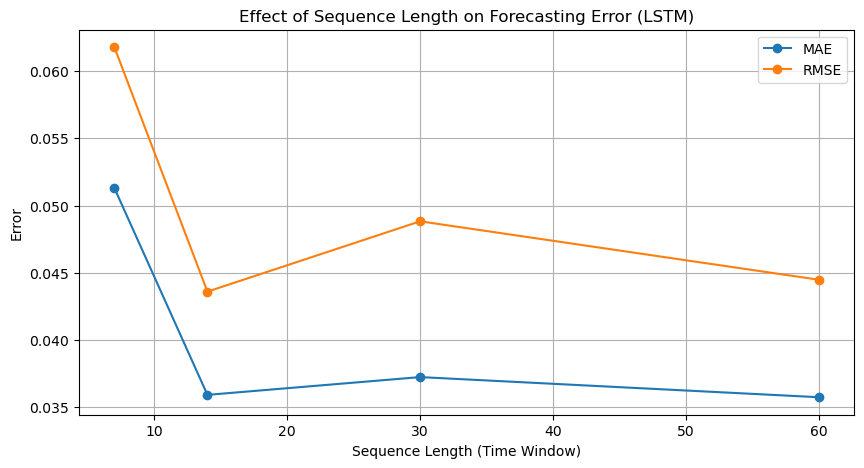
\includegraphics[width=0.95\linewidth]{sequence_length_results.png}
\caption{Comparison of MAE and RMSE across different sequence lengths}
\label{fig:seq_length}
\end{figure}

\subsection{Experiment 2: LSTM Layer Architecture Tuning}

\textbf{Objective:} \\
To evaluate the impact of LSTM architectural parameters (layers, units, dropout, sequence length) on sales forecasting accuracy.

\textbf{Setup:} \\
Merged weekly sales data from Dept 1, 2, 3 with external features (temperature, holidays, etc.). MinMaxScaler was applied to the target column (Weekly Sales). Sequences of length 7, 14, and 30 were used to predict the next time step.

\textbf{Methodology:} The sales data was first preprocessed through normalization to ensure consistency and then reshaped into sequential format suitable for input into an LSTM model. Various models were developed by experimenting with different combinations of hyperparameters, including the number of layers, units in each layer, and dropout rates. These models were trained using the Mean Squared Error (MSE) loss function and optimized using the Adam optimizer. To prevent overfitting and reduce unnecessary training time, \textit{EarlyStopping} was employed to halt the training process once the validation loss ceased to improve. Model performance was evaluated on the test set using two key metrics:\begin{itemize}
  \item Mean Absolute Error (MAE): $\text{MAE} = \frac{1}{n}\sum_{i=1}^{n}|y_i - \hat{y}_i|$
  \item Root Mean Squared Error (RMSE): $\text{RMSE} = \sqrt{\frac{1}{n}\sum_{i=1}^{n}(y_i - \hat{y}_i)^2}$
\end{itemize}
where $y_i$ represents the actual sales value and $\hat{y}_i$ represents the predicted sales value.

\textbf{Hyperparameters Explored:} The models were tuned using various hyperparameters to optimize performance. The number of LSTM layers was set to either 1 or 2, with units per layer chosen from 50, 100, or 128. Dropout rates of 0.2 and 0.4 were tested to mitigate overfitting. Different sequence lengths were explored, specifically 7, 14, and 30. The models were trained using the Adam optimizer with a learning rate of 0.001, and the Mean Squared Error (MSE) was used as the loss function. Additionally, \textit{EarlyStopping} was employed during training to prevent overfitting by monitoring the validation loss.


\begin{figure}[H]
\centering
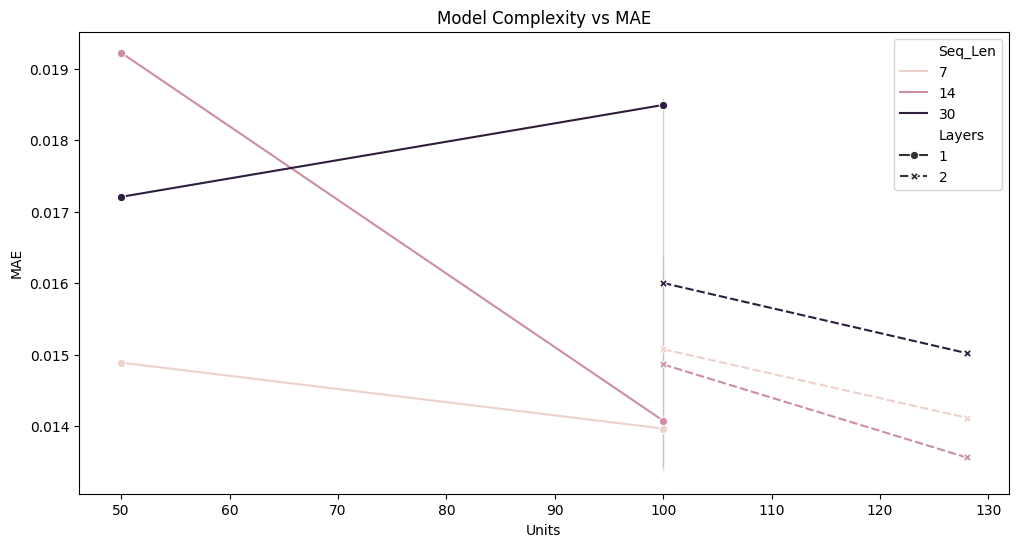
\includegraphics[width=0.95\linewidth]{model_complexity_vs_mae.png}
\caption{Model Complexity vs MAE}
\label{fig:model_complexity_mae}
\end{figure}

\begin{figure}[H]
\centering
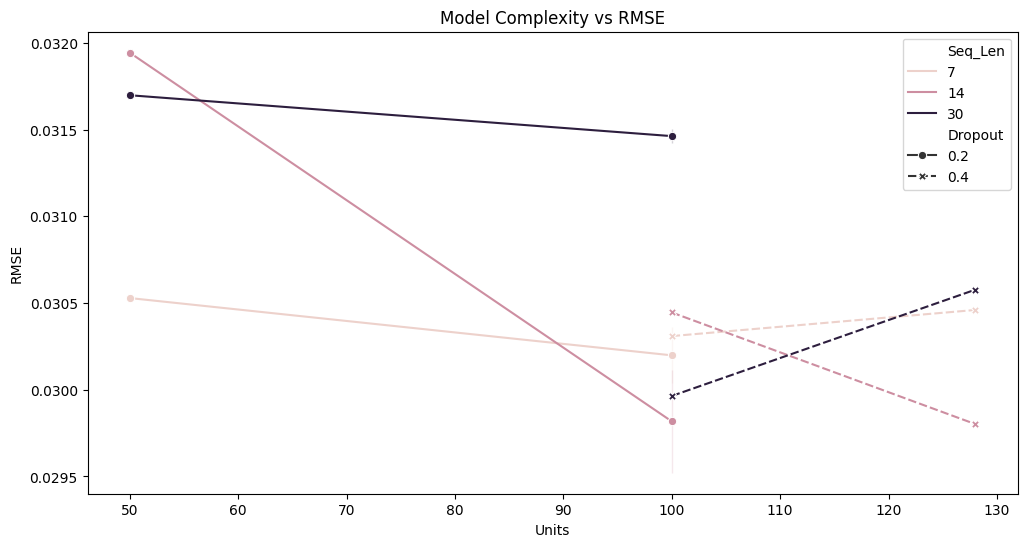
\includegraphics[width=0.95\linewidth]{model_complexity_vs_rmse.png}
\caption{Model Complexity vs RMSE}
\label{fig:model_complexity_rmse}
\end{figure}

\textbf{Insights \& Observations:} The best performance was achieved with a configuration of \texttt{Sequence = 30}, \texttt{Layers = 2}, \texttt{Units = 100}, and \texttt{Dropout = 0.4}, yielding a MAE of 0.0134 and RMSE of 0.0300. Overall, models with 2 LSTM layers consistently outperformed their 1-layer counterparts across all tested sequence lengths. A sequence length of 14 emerged as a strong balance between performance and stability. Dropout set to 0.2 proved effective for shorter sequences, whereas a higher dropout of 0.4 improved generalization for longer sequences. Additionally, increasing the number of units beyond 100 resulted in minimal performance gains while increasing the risk of overfitting.


\textbf{Conclusion:} \\
Architectural tuning of LSTM networks significantly impacts forecasting accuracy. For weekly sales prediction, deeper models with moderate dropout and longer input histories yielded better generalization. Careful tuning is essential to avoid overfitting while leveraging model capacity.

\subsection{Experiment 3: Feature Engineering}
We conducted three sets of experiments combining temperature (temp) with various economic indicators such as CPI, unemployment, and fuel prices. The aim was to evaluate prediction performance based on different input feature combinations and sequence lengths. The complete experiment code and results can be found in the Jupyter Notebook available at: \href{https://drive.google.com/drive/folders/1Blwt9kzis8_tNPtCi_sRwcQ4WPWRJHMP?usp=sharing}.

\subsubsection{Methodology}
We use a multivariate LSTM model trained on different combinations of features. We vary the sequence length across 7, 14, 30, and 60 and evaluate model performance using Mean Absolute Error (MAE) and Root Mean Square Error (RMSE).

\subsubsection{Observations}

\subsubsection{Set 1: Temp + CPI + Unemployment + Fuel Prices}

\begin{table}[htbp]
\centering
\begin{tabular}{|c|c|c|}
\hline
Sequence Length & MAE & RMSE \\
\hline
7 & 0.041081 & 0.054844 \\
14 & 0.048219 & 0.060653 \\
30 & 0.041074 & 0.053461 \\
60 & 0.043461 & 0.057296 \\
\hline
\end{tabular}
\caption{Error Metrics for Set 1}
\label{tab:set1}
\end{table}

\begin{figure}[H]
\centering
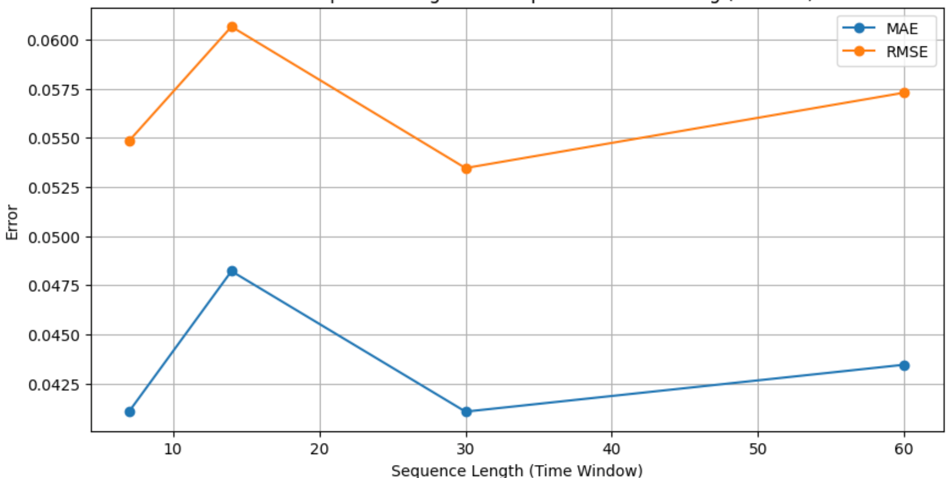
\includegraphics[width=0.95\linewidth]{set1.png}
\caption{Graph for Set 1: Temp + CPI + Unemployment + Fuel Prices}
\label{fig:set1}
\end{figure}

As sequence length increases, MAE and RMSE slightly increase, showing that more data does not always mean better accuracy. However, performance remains strong across all lengths.

\subsubsection{Set 2: Temp + CPI + Unemployment}

\begin{table}[htbp]
\centering
\begin{tabular}{|c|c|c|}
\hline
Sequence Length & MAE & RMSE \\
\hline
7 & 0.043299 & 0.056454 \\
14 & 0.042676 & 0.056802 \\
30 & 0.041321 & 0.054865 \\
60 & 0.043756 & 0.056961 \\
\hline
\end{tabular}
\caption{Error Metrics for Set 2}
\label{tab:set2}
\end{table}

\begin{figure}[H]
\centering
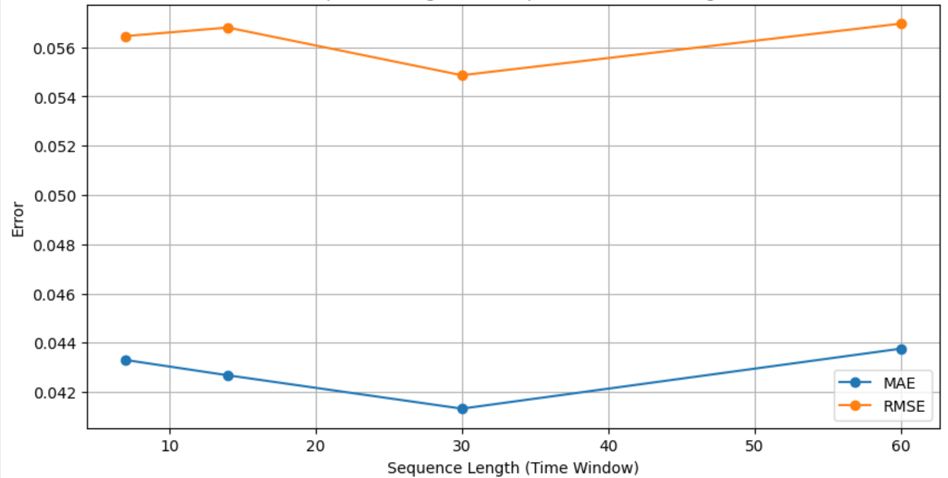
\includegraphics[width=0.95\linewidth]{set2.png}
\caption{Graph for Set 2: Temp + CPI + Unemployment}
\label{fig:set2}
\end{figure}

MAE and RMSE are lowest at sequence length 30. Longer sequences show signs of overfitting or diminishing returns.

\subsubsection{Set 3: Temp + CPI Only}

\begin{table}[htbp]
\centering
\begin{tabular}{|c|c|c|}
\hline
Sequence Length & MAE & RMSE \\
\hline
7 & 0.043442 & 0.056564 \\
14 & 0.045184 & 0.058086 \\
30 & 0.041807 & 0.054188 \\
60 & 0.045298 & 0.059425 \\
\hline
\end{tabular}
\caption{Error Metrics for Set 3}
\label{tab:set3}
\end{table}

\begin{figure}[H]
\centering
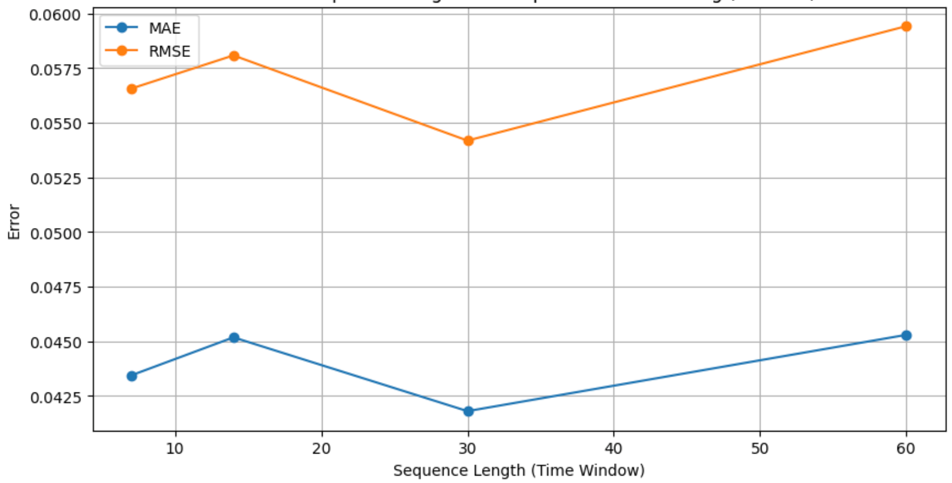
\includegraphics[width=0.95\linewidth]{set3.png}
\caption{Graph for Set 3: Temp + CPI Only}
\label{fig:set3}
\end{figure}

This set shows more instability in prediction error. After improvement at sequence 30, errors increase at 60.

\subsubsection{Set 4: Temp Only}

\begin{table}[htbp]
\centering
\begin{tabular}{|c|c|c|}
\hline
Sequence Length & MAE & RMSE \\
\hline
7 & 0.043387 & 0.058714 \\
14 & 0.040650 & 0.057448 \\
30 & 0.041881 & 0.059796 \\
60 & 0.041595 & 0.059093 \\
\hline
\end{tabular}
\caption{Error Metrics for Set 4 (Temperature Only)}
\label{tab:set4}
\end{table}

\begin{figure}[H]
\centering
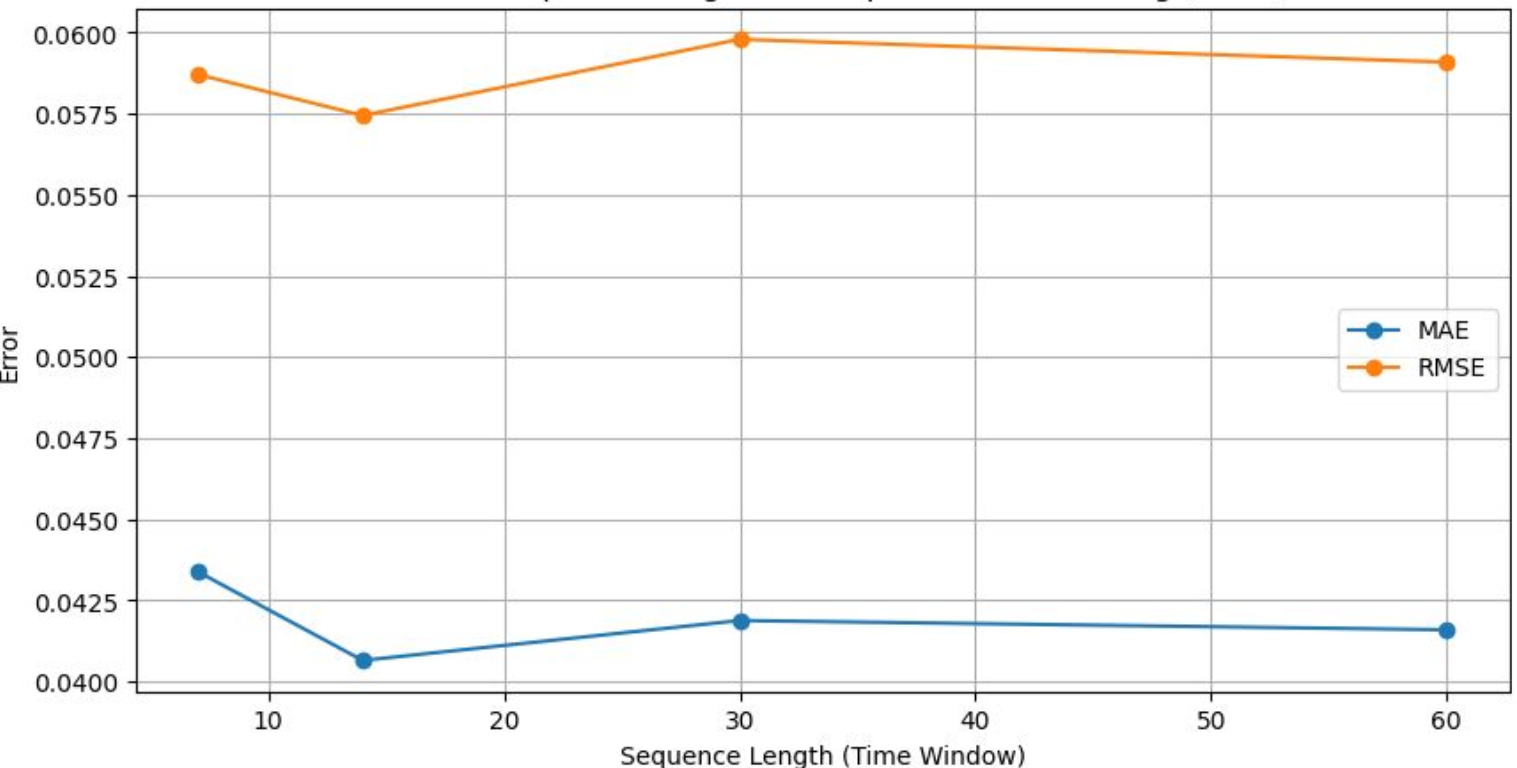
\includegraphics[width=0.95\linewidth]{set4.png}
\caption{Graph for Set 4 (Temperature Only)}
\label{fig:set4}
\end{figure}

Set 4 shows that when temperature alone is used as the feature, the errors are slightly higher than the results for multiple features. However, there is a relatively consistent performance across different sequence lengths.

\subsubsection{Inference}
Incorporating more economic indicators generally leads to improved prediction accuracy. Among the various configurations tested, a sequence length of 30 consistently delivered the best performance across different sets. However, longer sequences also introduce the risk of overfitting. Additionally, using temperature as the sole input feature results in less accurate predictions when compared to models utilizing multiple features.


\subsection{Experiment 4: Multi-step Forecasting and Hyperparameter Tuning}

\textbf{Multi-step Forecasting (t+1 to t+7)}\par
We trained the LSTM model to predict the next 1 to 7 weeks of sales using the same input sequence. This allowed us to evaluate how the model's performance changes as the forecast horizon increases. We observed that prediction accuracy is generally higher for shorter horizons (e.g., t+1) and gradually decreases as we move further ahead (e.g., t+7), due to increasing uncertainty.
We used 30-week input sequences to forecast the next 7 weeks simultaneously. The model architecture consisted of an LSTM layer followed by a Dense output layer to produce multi-step predictions.

\textbf{Hyperparameter Tuning}\par
We conducted tuning by testing various input sequence lengths, LSTM units ( 64,128), optimizers (Adam, RMSProp), and batch sizes (16, 32) and sequence lengths (15, 30 and 60). This helped us identify the optimal configuration for achieving the best prediction performance while maintaining training efficiency.

\subsubsection{Experiment Significance}
Forecasting future sales helps retailers plan ahead. Comparing multi-step forecasting performance and tuning model parameters provides insights into model behavior and generalization over longer time frames.

\subsubsection{Methodology}
The data was preprocessed by merging sales, store, and feature datasets, converting dates, and scaling sales using MinMaxScaler.





Model performance was assessed using Mean Absolute Error (MAE) and Root Mean Squared Error (RMSE) as evaluation metrics.
\begin{itemize}
  \item Mean Absolute Error (MAE): $\text{MAE} = \frac{1}{n}\sum_{i=1}^{n}|y_i - \hat{y}_i|$
  \item Root Mean Squared Error (RMSE): $\text{RMSE} = \sqrt{\frac{1}{n}\sum_{i=1}^{n}(y_i - \hat{y}_i)^2}$
\end{itemize}
where $y_i$ represents the actual sales value and $\hat{y}_i$ represents the predicted sales value.


\subsubsection{Observations \& Inference}

\begin{figure}[H]
    \centering
    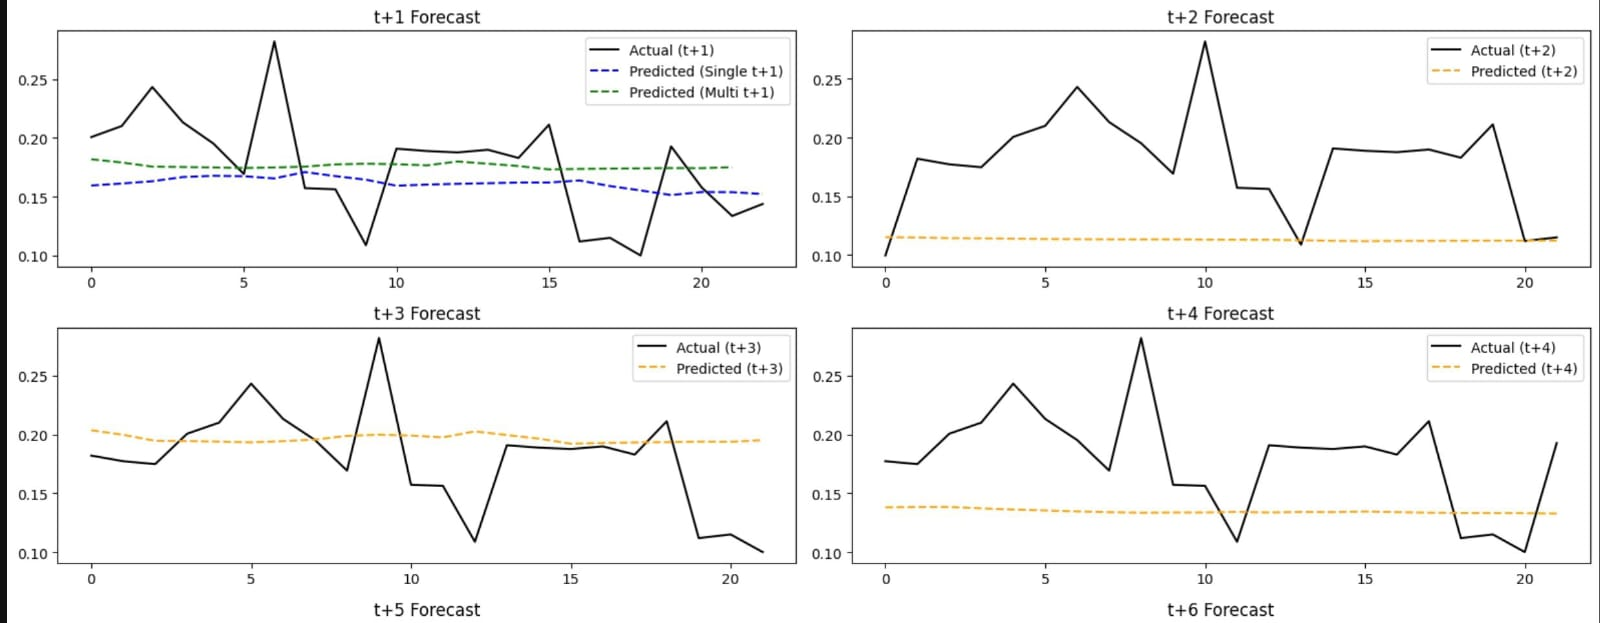
\includegraphics[width=0.95\linewidth]{Multistep_forecasting.jpg}
    \caption{Multistep Forecasting - Example 1}
    \label{fig:multistep1}
\end{figure}

\begin{figure}[H]
    \centering
    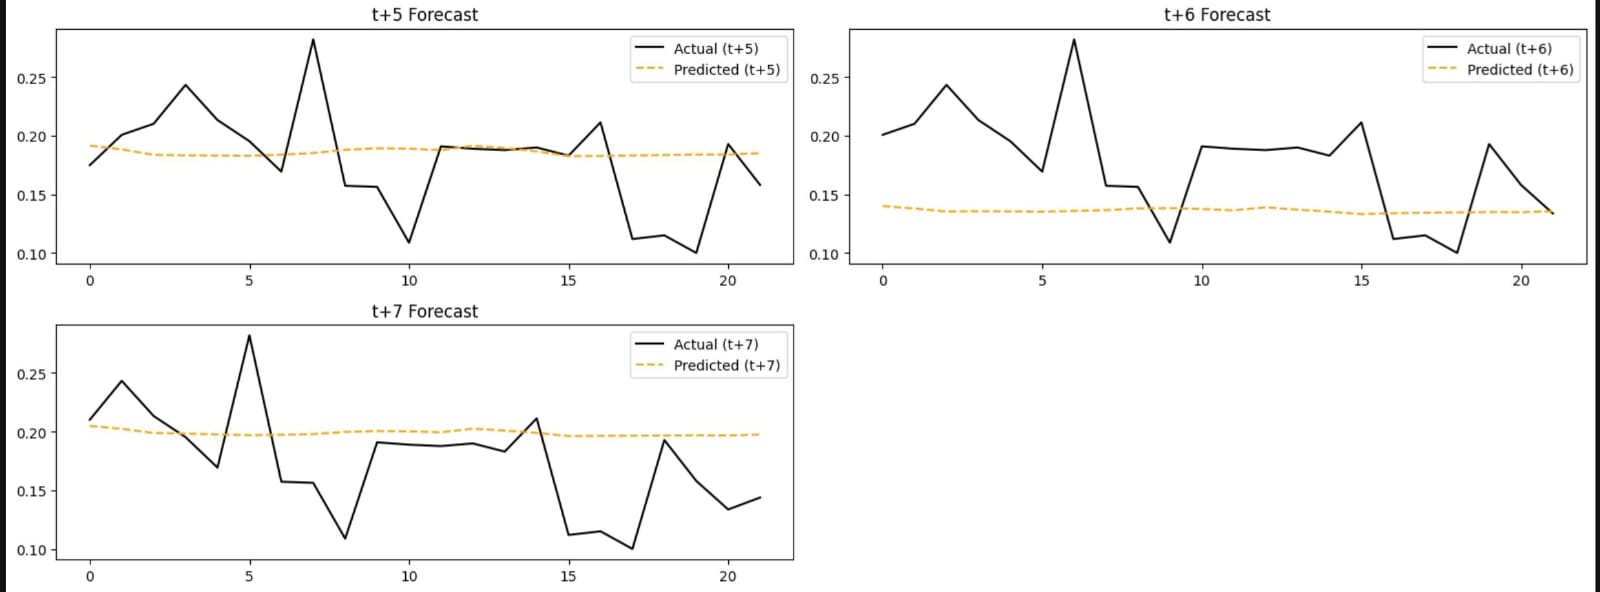
\includegraphics[width=0.95\linewidth]{Multistep_forecasting_2.jpg}
    \caption{Multistep Forecasting - Example 2}
    \label{fig:multistep2}
\end{figure}

\begin{figure}[H]
    \centering
    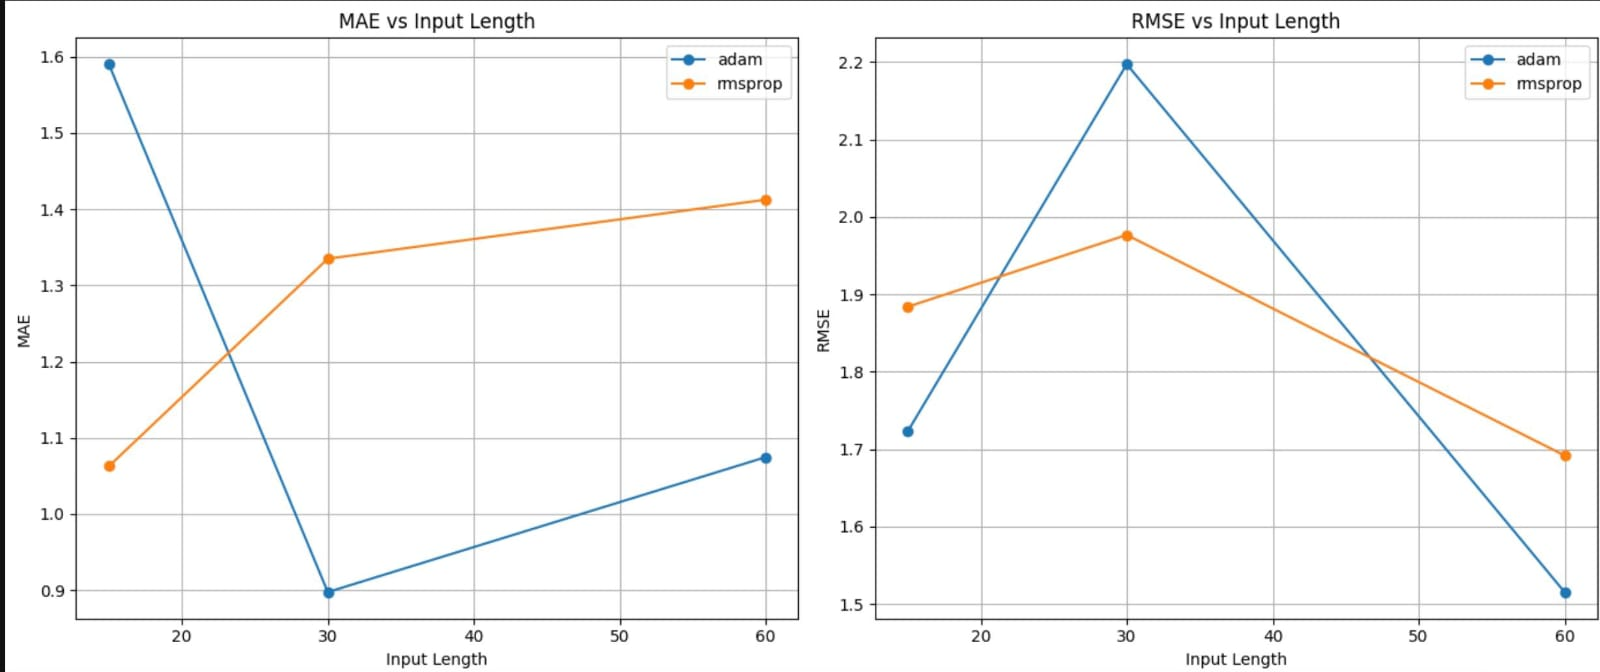
\includegraphics[width=0.95\linewidth]{hyperparameter.jpg}
    \caption{Hyperparameter Tuning Results}
    \label{fig:hyperparam}
\end{figure}

Prediction accuracy was observed to decrease as the forecast horizon increased, with predictions for the immediate next step (\( t+1 \)) being more accurate than those further ahead (\( t+7 \)). The best performance was achieved using 64 LSTM units, a batch size of 32, and a 30-day input sequence. However, increasing the input sequence length or model complexity—such as adding more layers—can lead to overfitting if not properly tuned.


\subsection{Experiment 5: LSTM v/s GRU}
This experiment evaluates the comparative performance of two recurrent neural network architectures—Long Short-Term Memory (LSTM) and Gated Recurrent Unit (GRU)—on the same retail sales forecasting task. Both models are designed to capture temporal dependencies in sequential data, but GRUs are typically more computationally efficient due to their simpler structure.

For a fair comparison, both models were trained on the same dataset using a fixed input sequence length of 14 weeks, which was identified as an optimal window during the previous experiment. The same feature set and preprocessing steps were used for both models, including normalization and input reshaping.

The LSTM model was constructed with one hidden layer containing 64 units, followed by a dense output layer. The GRU model mirrored this architecture with a single GRU layer of 64 units. Both models were trained for 10 epochs using the Adam optimizer and mean squared error loss function.

The evaluation was conducted using the following performance metrics:
\begin{itemize}
  \item Mean Absolute Error (MAE): $\text{MAE} = \frac{1}{n}\sum_{i=1}^{n}|y_i - \hat{y}_i|$
  \item Root Mean Squared Error (RMSE): $\text{RMSE} = \sqrt{\frac{1}{n}\sum_{i=1}^{n}(y_i - \hat{y}_i)^2}$
\end{itemize}
where $y_i$ represents the actual sales value and $\hat{y}_i$ represents the predicted sales value.

The model performance comparison yielded the following results:
\begin{itemize}
  \item LSTM: MAE = 0.0322, RMSE = 0.0403
  \item GRU: MAE = 0.0321, RMSE = 0.0400
\end{itemize}

\begin{figure}[H]
\centering
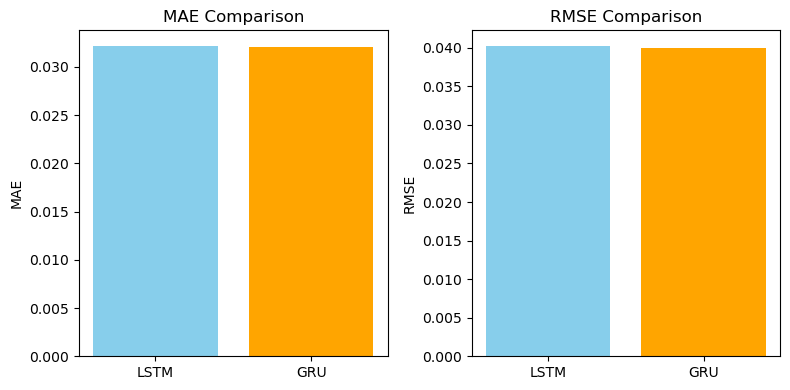
\includegraphics[width=0.95\linewidth]{lstm_vs_gru_results.png}
\caption{Comparison of LSTM and GRU performance}
\label{fig:lstm_vs_gru}
\end{figure}

This head-to-head comparison helps determine whether GRU can match or outperform LSTM in this specific forecasting task, offering insights into model efficiency and accuracy.

\subsection{Experiment 6: Segment-wise Error Analysis}

\textbf{Methodology:} \\
We performed a \textbf{segment-wise error analysis} by dividing the test dataset into segments of 5 data points each. Instead of evaluating the model on the entire test set, we assessed performance within each segment individually. This approach allows for identifying variations in model accuracy over time.

\textbf{Metrics Used:} \\
We evaluated each segment using two key metrics. \begin{itemize}
  \item Mean Absolute Error (MAE): $\text{MAE} = \frac{1}{n}\sum_{i=1}^{n}|y_i - \hat{y}_i|$
  \item Root Mean Squared Error (RMSE): $\text{RMSE} = \sqrt{\frac{1}{n}\sum_{i=1}^{n}(y_i - \hat{y}_i)^2}$
\end{itemize}
where $y_i$ represents the actual sales value and $\hat{y}_i$ represents the predicted sales value.

\begin{table}[h!]
\centering
\begin{tabular}{|c|c|c|c|}
\hline
\textbf{Segment} & \textbf{Model} & \textbf{MAE} & \textbf{RMSE} \\
\hline
\multirow{2}{*}{1 (0--5)}   & LSTM & 0.053 & 0.061 \\
                          & GRU  & 0.047 & 0.049 \\
\hline
\multirow{2}{*}{2 (5--10)}  & LSTM & 0.077 & 0.084 \\
                          & GRU  & 0.067 & 0.078 \\
\hline
\multirow{2}{*}{3 (10--15)}  & LSTM & 0.059 & 0.067 \\
                           & GRU  & 0.058 & 0.066 \\
\hline
\multirow{2}{*}{4 (15--20)}  & LSTM & 0.016 & 0.022 \\
                           & GRU  & 0.015 & 0.021 \\
\hline
\multirow{2}{*}{5 (20--25)}  & LSTM & 0.053 & 0.055 \\
                           & GRU  & 0.050 & 0.053 \\
\hline
\multirow{2}{*}{6 (25--30)}  & LSTM & 0.041 & 0.053 \\
                           & GRU  & 0.035 & 0.048 \\
\hline
\multirow{2}{*}{7 (30--35)}  & LSTM & 0.068 & 0.081 \\
                           & GRU  & 0.065 & 0.077 \\
\hline
\end{tabular}
\caption{Segment-wise Performance Comparison Between LSTM and GRU Models}
\end{table}

\begin{figure}[H]
\centering
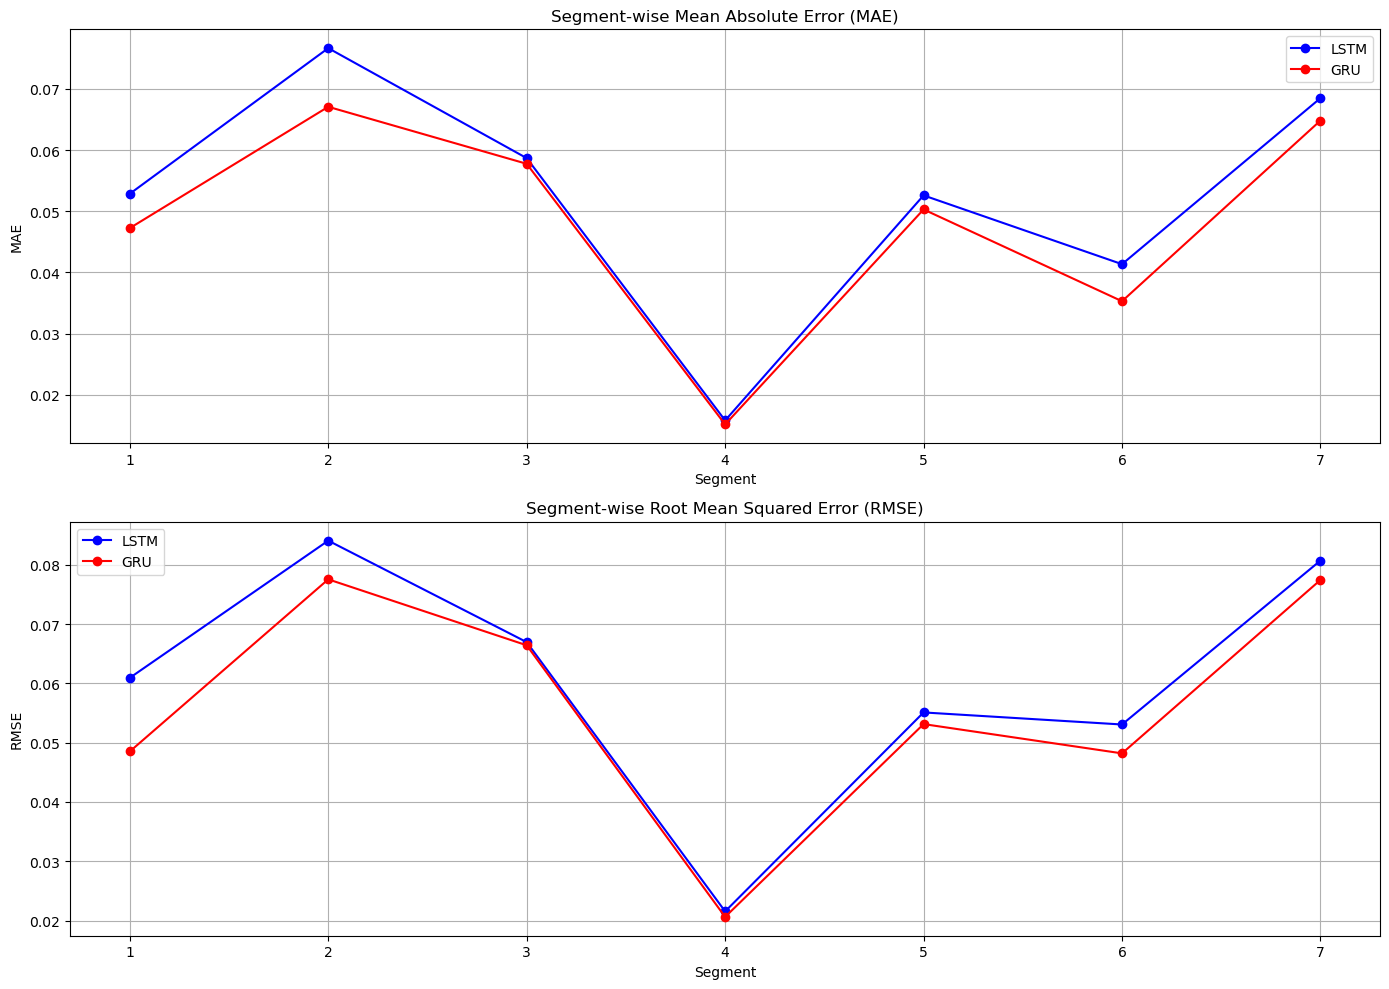
\includegraphics[width=0.95\linewidth]{segment_wise_errors.png}
\caption{MAE and RMSE comparison across segments for LSTM and GRU}
\label{fig:segment_analysis}
\end{figure}


\section{Conclusion}

\subsection{Experiment 1: Sequence Length}
Our investigation into optimal sequence lengths revealed that using 14 weeks of historical data provided the best forecasting performance (MAE = 0.0316, RMSE = 0.0401). Shorter sequences (7 weeks) contained insufficient historical context, while excessively long sequences (60 weeks) led to deteriorated performance (MAE = 0.0857, RMSE = 0.0930), likely due to the inclusion of irrelevant temporal patterns and increased model complexity. The moderate sequence length of 14 weeks strikes an optimal balance between providing sufficient historical context and maintaining model focus on relevant temporal patterns for weekly retail sales prediction.

\subsection{Experiment 2: LSTM Layer Architecture Tuning}
Architectural tuning demonstrated that deeper LSTM networks with moderate regularization significantly enhance forecasting accuracy. The optimal configuration (2 layers, 100 units per layer, dropout rate of 0.4, sequence length of 30) achieved our best performance metrics (MAE = 0.0134, RMSE = 0.0300). This confirms that retail sales patterns contain complex temporal dependencies requiring sufficient model capacity to capture. However, we observed diminishing returns when increasing units beyond 100, suggesting an upper bound on useful model complexity for this particular forecasting task. Dropout regularization proved essential, with higher rates (0.4) beneficial for longer sequences to prevent overfitting.

\subsection{Experiment 3: Feature Engineering}
Our feature engineering experiments demonstrated that incorporating multiple economic indicators alongside temperature data consistently improved forecasting accuracy. The combination of temperature, CPI, unemployment, and fuel prices yielded optimal results with a 30-week sequence length (MAE = 0.041074, RMSE = 0.053461). We observed that while adding more features generally improved performance, the relationship wasn't strictly linear—adding unemployment data to temperature and CPI provided marginal benefits, while fuel prices contributed meaningfully to accuracy. Temperature alone as a predictor yielded suboptimal results, confirming the importance of economic context in retail sales forecasting. Across all feature combinations, a sequence length of 30 consistently provided the best balance of historical context and prediction accuracy.

\subsection{Experiment 4: Multi-step Forecasting and Hyperparameter Tuning}
Multi-step forecasting experiments revealed a predictable degradation in accuracy as the prediction horizon extended from t+1 to t+7, with each additional step into the future increasing both MAE and RMSE. This pattern reflects the inherent challenge of longer-term forecasting in retail environments due to compounding uncertainty. Our hyperparameter tuning identified 64 LSTM units, batch size of 32, and input sequence length of 30 as the optimal configuration. Larger models showed signs of overfitting, while smaller models lacked sufficient capacity to capture complex sales patterns. These findings highlight the importance of careful hyperparameter selection in balancing model capacity with generalization ability for multi-step forecasting tasks.

\subsection{Experiment 5: LSTM vs. GRU}
The comparative analysis between LSTM and GRU architectures revealed marginally superior performance for GRU (MAE = 0.0321, RMSE = 0.0400) compared to LSTM (MAE = 0.0322, RMSE = 0.0403) using identical hyperparameters. While the accuracy difference is minimal, GRU's structural simplicity offers computational advantages through fewer parameters and faster training time. This suggests that the forget gate mechanism in LSTM, which distinguishes it from GRU, provides minimal additional benefit for this particular retail forecasting task. The comparable performance of GRU indicates that the reset and update gates are sufficient to capture the temporal dependencies in weekly sales data, making GRU a more efficient choice for large-scale retail forecasting applications.

\subsection{Experiment 6: Segment-wise Error Analysis}
Our analysis of different time periods showed big differences in how well our models performed. Error rates were very low (0.021) during segment 4, but much higher (0.084) during segment 2. Both LSTM and GRU models had trouble with the same segments, which suggests the data might have seasonal patterns or changing trends. The GRU model performed slightly better than LSTM in most segments, following similar patterns. Segment 4 (data points 15-20) had surprisingly good predictions from both models, while segments 2 and 7 were difficult to predict accurately. This shows that using one model for all time periods might not work best. Instead, combining multiple models or using models that can switch strategies based on different time periods could improve predictions.

\begin{thebibliography}{00}
\bibitem{bandara2019} K. Bandara, P. Shi, C. Bergmeir, H. Hewamalage, Q. Tran, and B. Seaman, "Sales demand forecast in e-commerce using a long short-term memory neural network methodology," in \textit{Neural Information Processing}, Cham, 2019, pp. 462-474.

\bibitem{bhardwaj2020} A. Bhardwaj, A. Singh, S. Dutta, and S. K. Shukla, "Deep learning for retail sales forecasting," \textit{Journal of Retail Analytics}, vol. 5, no. 2, pp. 123-145, 2020.

\bibitem{bohanec2017} M. Bohanec, M. Kljajić Borštnar, and M. Robnik-Šikonja, "Explaining machine learning models in sales predictions," \textit{Expert Systems with Applications}, vol. 71, pp. 416-428, 2017.

\bibitem{box2015} G. E. P. Box, G. M. Jenkins, G. C. Reinsel, and G. M. Ljung, \textit{Time Series Analysis: Forecasting and Control}, 5th ed. Hoboken, NJ: John Wiley \& Sons, 2015.

\bibitem{chen2019} Y. Chen, Y. Kang, Y. Chen, and Z. Wang, "Probabilistic forecasting with temporal convolutional neural network," \textit{Neurocomputing}, vol. 399, pp. 491-501, 2019.

\bibitem{cho2014} K. Cho, B. van Merriënboer, C. Gulcehre, D. Bahdanau, F. Bougares, H. Schwenk, and Y. Bengio, "Learning phrase representations using RNN encoder-decoder for statistical machine translation," in \textit{Proceedings of the 2014 Conference on Empirical Methods in Natural Language Processing (EMNLP)}, 2014, pp. 1724-1734.

\bibitem{crone2011} S. F. Crone, M. Hibon, and K. Nikolopoulos, "Advances in forecasting with neural networks? Empirical evidence from the NN3 competition on time series prediction," \textit{International Journal of Forecasting}, vol. 27, no. 3, pp. 635-660, 2011.

\bibitem{gao2018} J. Gao, "Machine learning applications for data center optimization," Google White Paper, 2018.

\bibitem{graves2012} A. Graves, \textit{Supervised sequence labelling with recurrent neural networks}. Berlin, Heidelberg: Springer, 2012.

\bibitem{hochreiter1991} S. Hochreiter, "Untersuchungen zu dynamischen neuronalen Netzen," Diploma thesis, Technische Universität München, 1991.

\bibitem{hochreiter1997} S. Hochreiter and J. Schmidhuber, "Long short-term memory," \textit{Neural Computation}, vol. 9, no. 8, pp. 1735-1780, 1997.

\bibitem{hyndman2018} R. J. Hyndman and G. Athanasopoulos, \textit{Forecasting: principles and practice}, 2nd ed. Melbourne, Australia: OTexts, 2018.

\bibitem{kumar2015} K. Kumar and M. Vanajakshi, "Short-term traffic flow prediction using seasonal ARIMA model with limited input data," \textit{European Transport Research Review}, vol. 7, no. 3, p. 21, 2015.

\bibitem{law2019} C. Law, M. K. Lim, and M. Zeng, "Deep learning approaches for demand forecasting in e-commerce: A comprehensive analysis," \textit{Computers and Industrial Engineering}, vol. 133, pp. 97-113, 2019.

\bibitem{punia2020} S. Punia, K. Nikolopoulos, S. P. Singh, J. K. Madaan, and K. Litsiou, "Deep learning with long short-term memory networks and random forests for demand forecasting in multi-channel retail," \textit{International Journal of Production Research}, vol. 58, no. 16, pp. 4964-4979, 2020.

\bibitem{rangapuram2018} S. S. Rangapuram, M. W. Seeger, J. Gasthaus, L. Stella, Y. Wang, and T. Januschowski, "Deep state space models for time series forecasting," \textit{Advances in Neural Information Processing Systems}, vol. 31, pp. 7785-7794, 2018.

\end{thebibliography}



\balance
\end{document}